\chapter{More About Configuring MATSim}
\label{ch:configuring}
% ##################################################################################################################

\hfill \textbf{Author:} Andreas Horni, Kai Nagel

\begin{center} 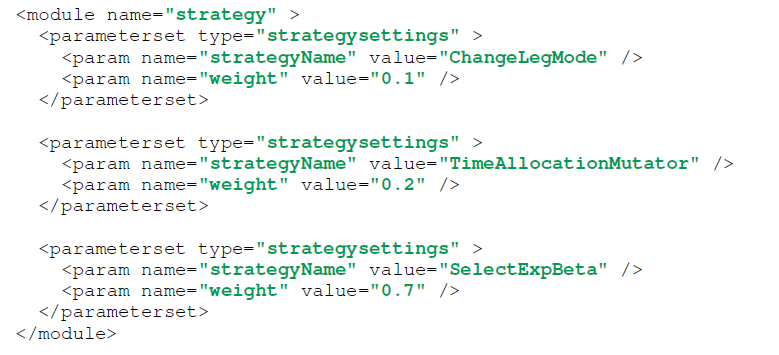
\includegraphics[width=0.3\textwidth, angle=0]{using/figures/strategy.png} \end{center}

\editdone{This text has undergone the professional edit. Please no grammatical changes anymore! They are most-probably wrong.}

% ##################################################################################################################
This chapter describes configuration options that can be used together with the three basic elements: \gls{configfile}, population and network.
%are exclusively done by the \gls{configfile}. \gls{matsim} configuring  requiring
%% Aspects that require further input data are described in Chapter~\ref{ch:modules}. The technical details for module usage, in particular the parameter sets are described in \citep[][]{MATSim_Userguide_2015} and in the \gls{javadoc}.
%
Part~\ref{part:extending-matsim} discusses various options to extend \gls{matsim} beyond these three elements, sometimes using only additional files, or using additional \gls{jar} files beyond the \gls{matsim} core \gls{jar} file, or by writing so-called ``scripts in \gls{java}'', or by adding or replacing functionality.

\gls{matsim} writes configuration files in several location; for example, in the logfile, in the iteration output directory, or the \lstinline{CreateFullConfig} functionality described in Section~\ref{sec:lgs-config}.  As explained in Section~\ref{sec:survival}, these files come with comments explaining configuration options.  This is often the best source for configuration options.  %\kai{Andreas, meinem Eindruck nach geht der user guide hier auch nicht weiter als das Buch -- und soll es derzeit auch gar nicht.  Unsere Javadoc sagt m.E.\ traditionell sehr wenig bis gar nichts über config.} \ah{ok}

% ##################################################################################################################
\section{MATSim Data Containers}
\label{sec:using-data-containers}
%% \kai{Eigentlich steht das alles schon in Section~\ref{sec:inputdata}.  Ist es wirklich sinnvoll, das zu doppeln?  Oder schreiben wir hier halt die ``weiteren'' Container rein (dann sollten wir aber einiges weitere von oben hier runter holen).}
%% \ah{M.E. jetzt ok.}

% ===================================================================================
\subsection{Network}
\label{sec:using-network}
The \gls{configfile} section \lstinline|network|
%amongst other
specifies which network file will be used in the simulation (Section~\ref{sec:lgs-config} and \ref{sec:lgstarted-network-file}). Further configuration options, \eg specification of time-variant networks, are presented in Section~\ref{sec:extending-network}.

% ===================================================================================
\subsection{Population}
\label{sec:using-population}
The \gls{configfile} section \lstinline|plans| allows population specifiction with its day plans (Section~\ref{sec:lgs-config} and \ref{sec:lgstarted-population-file}). Further configuration options, \eg specification of arbitrary agent attributes or subpopulations, are presented in Section~\ref{sec:extending-population}.

Further \gls{matsim} containers are described in Section~\ref{sec:extending-data-containers}.

%##################################################################################################################
\section{Global Modules and Global Aspects}
\label{sec:using-globalmodules}
% ===================================================================================
\subsection{Controler}
\label{sec:using-controler}
The controler is an indispensable module for running \gls{matsim}; its parameters are set in the \lstinline|controler| \gls{configfile} section. The \gls{matsimrun}'s output directory, its number of iterations and the plans and events ouput interval can be specified here. and the expected \gls{mobsim} can be defined (Section~\ref{sec:using-mobsims}). Importantly, the routing algorithm is defined here by using
%
\begin{xml}
<module name="controler" >
    <param name="routingAlgorithmType" value="{Dijkstra | FastDijkstra |
    		AStarLandmarks | FastAStarLandmarks}" />
    [...]
</module>
\end{xml}
%
%In Section~\ref{sec:extending-controler}, the
Possibilities for extending the \lstinline|Controler| functionality is given in %Section~\ref{sec:extending-controler} and % da steht nichts mehr. kai, jan'15
Chapter~\ref{ch:extensionpoints}.

% ===================================================================================
\subsection{Events}
\label{sec:using-events}

Events are continuously generated, reporting on all activities in the \gls{mobsim}, as discussed in more detail in Section~\ref{sec:events-extension-point}. 
%% The core module, not having its own \gls{configfile} section, also contains readers and writers.
% 
% I don't think that the above sentence is interesting at the "using" level. kai, mar'15

% ===================================================================================
\subsection{Parallel Computing}
\label{sec:using-parallel-computing}

\gls{matsim} uses multi-threading to accelerate computing speeds.  Related configuration parameters can be found in several config modules; they are combined into one section here.

% ...................................
\paragraph{Global Setting}

The \lstinline{global} section contains
\begin{xml}
<module name="global" >
    <param name="numberOfThreads" value="2" />
    [...]
</module>
\end{xml}
This number is used in several places; most importantly, innovative strategies, where multiple routing requests are distributed to multiple threads.

A good starting point is using the number of available cores.

% ...................................
\paragraph{Parallel Event Handling}
\label{sec:using-paralleleventhandling}

The \gls{configfile} section \lstinline|parallelEventHandling| is used to define the number of threads used for event handling. 
As described in \citet[][]{WaraichEtAl_STRC_2009}, the simulation can be substantially accelerated when using multiple threads for the events handling, which can be a bottleneck in \gls{matsim} simulation runs.
% Clearly, the number of threads should correspond with available processor cores.  \kai{Meine Erfahrung ist eine andere, und je nach Maschine kann man das manchmal überauslasten und manchmal sollte man es eher unterauslasten.}  
%% In our experience, the optimal degree of capacity utilization (threads versus cores) is highly machine-dependent.
%% As mentioned above, the \gls{mobsim} \gls{qsim} is running parallel by default.

%% Being able to speed up scenarios might become even more important in the future, when additional innovation (choice) dimensions are added with large parameter variability, necessitating ensemble runs. % (see Section~\ref{sec:variability}).

% ...................................
\paragraph{Parallel QSim}

The number of threads for the parallel \gls{qsim} (\cf \cite{Dobler_PhDThesis_2013}) can be configured by
\begin{xml}
<module name="qsim" >
    <param name="numberOfThreads" value="10" />
    [...]
</module>
\end{xml}

%\ah{Marcel hatte mal Testreihe mit Identifikation der Laufzeit einzelner Module (QSim, Eventshandling etc.) geplant. Nachfragen, ob schon was vorhanden}

% ...................................
\paragraph{General Recommendations}

Generally, computations using threads are not necessarily faster with more threads, which is also true for \gls{matsim}. Some experimentation is necesary for each combination of scenario and hardware.  Here are some recommendations:
\begin{itemize}\styleItemize

\item For the ``global'' number of threads, a good starting point is the number of available cores.

\item It is no longer possible to switch off parallel event handling completely; setting it to `0' or `null' or `1' eventually achieves the same result.  Setting it to values larger than one sometimes leads to performance gains, but they are rarely significant.

\item The most sensitive parameter is that for the \gls{qsim}.
  %
  For somewhat older hardware (\eg Apple Macbook Pro from~2010), using all three remaining cores -  in addition to the parallel event handling - led to negligible performance gains and left the machine useless, even for normal office tasks.
  %
  For new hardware (\eg Apple Macbook Pro from~2014), using six of the available eight cores for the \gls{qsim} can make the \gls{mobsim} more than a factor of two faster and the machine can still be used for office tasks.
  %
  Experiences with older servers shows that one must carefully investigate the number of threads for the \gls{mobsim}, since using more threads often slows it down \citep{Dobler_PhDThesis_2013}.
  %
  No experiences with new servers are currently available. 
%% \kai{or are there?  where?} \ah{Gemäss Patrick ist Sergio was am Basteln mit Desktop-Clustern.}
  \item High Performance Computing Clusters are often available to researchers, allowing access to high quality machines with reduced management overhead. Typically, one pays for computation time, either directly, or by a loss of priority, with an amount proportional to the reserved resources, that is, the time the job took to finish, multiplied by the number of reserved cores. In this kind of situation, the number of cores used throughout the whole process should be stable, to avoid paying for unused resources. A recommendation in this case is thus to set the number of threads for the QSim to the best value $n$ (see above) and then set the ``global'' number of threads to this same $n$, and submit the job requesting $n$ cores.
	  Also note that fewer threads are almost always better, in terms of throughput.
	  In addition, for both calibration and ``what-if'' scenario exploration,
	  one typically needs to run a large number of simulations with different parameters or
	  input data.
	  As total RAM memory is usually not an issue on a cluster,
	  it is often more efficient to run a large number of simulations simultaneously
	  with a low number of threads, rather than a low number of simulations with lots of threads.

\end{itemize}

%% \kai{number of threads: nicht unter parallel computing?  Wäre meiner Erfahrung nach tatsächlich hilfreich, die paralellen Aspekte zusammenzufassen.} \ah{\url{https://matsim.atlassian.net/browse/MATSIM-310}} \kai{Ich meinte eigentlich eher, sie ``im Buch'' zusammen zu fassen.  Im code scheint mir das derzeit nicht genügende Priorität zu haben, zumal wir mit dem Buch langsam in die Zielgerade kommen müssen.  Bin mir auch nicht sicher, ob wir das im code wirklich umbauen wollen. }


% ===================================================================================
\subsection{Global}
\label{sec:using-global}
In the \gls{configfile} section \lstinline|global|, the simulation's random seed, the ``global'' number of \gls{java} threads (see above) and the coordinate system (\cf Section~\ref{sec:unitsconventions}) can be defined. 

% ##################################################################################################################
\section{Mobility Simulations}
\label{sec:using-mobsims}
An overview of \gls{matsim} mobility simulations is given in \citet[][]{Dobler_TechRep_IVT_2011}. %See also \citet[][]{Rieser_unpub_IVT_2011}.

% ===================================================================================
\subsection{\protect\gls{qsim}}
\label{sec:using-qsim}
The queue-based and time-step based \gls{qsim} \citep[][]{Gawron_IJMPC_1998,SimonEtAl_IJMPC_1999,CetinBurriNagel2003queue,Dobler_TechRep_IVT_2011, Dobler_STRC_2010} is \gls{matsim}'s default \gls{mobsim}. 
Its parameters are set in the \lstinline|qsim| \gls{configfile} section. Important parameters are:
%% \begin{itemize} 
%% \item
By specifying
\begin{xml}
   <param name="numberOfThreads" value="..."/>
\end{xml}
\gls{qsim} can be run in parallel, see Section~\ref{sec:using-parallel-computing}. 
%
%% \item 
Importantly, the \lstinline{qsim} parameters
\begin{xml}
    <param name="flowCapacityFactor" value="..." />
    <param name="storageCapacityFactor" value="..." />
\end{xml}
need to be set accordingly when running sample scenarios. For example, for a 10\,\% sample, these factors need to be 0.1. The \gls{matsim} \gls{gui} (Figure~\ref{fig:matsimgui}) allows adaptation of these parameters with the command \lstinline|Tools...Create Sample Population|.
%
%% \item
The link dynamics, either \gls{fifo} or passing can be specified by the parameter 
\begin{xml}
   <param name="linkDynamics" value="..." />
\end{xml}
%
%\item
Currently \gls{qsim} is implemented as a single-queue simulation queue (see Chapter~\ref{ch:kinematicwaves}), \ie back-propagating gaps as discussed in Section~\ref{sec:trafficflowmodel} are only available experimentally; 
they will be added soon (see Section~\ref{sec:researchavenues-double-queue-mobsim}) and will then be configurable with the parameter
\begin{xml}
   <param name="trafficDynamics" value="..." />
\end{xml}
%% \kai{Das gibt es immer noch nicht wirklich.  Habe jetzt Amit rekrutiert, damit er mir da hoffentlich hilft.}
%% \ah{ok. angepasst}
%% \end{itemize}
%
As shown in Section~\ref{sec:using-qsim-multimodal}, \gls{qsim} can handle \gls{multimodal} scenarios. %% \kai{chk}

%% \ah{explizit hinzufügen ist jetzt nicht mehr nötig, weil default, oder?}
%% To invoke \gls{qsim}, the parameter \lstinline|mobsim| of \lstinline|controler| \gls{configfile} section must be set to \lstinline|qsim| and a \lstinline|qsim| \gls{configfile} section must be provided.
%% \kai{ja, qsim ist default.}

% ===================================================================================
\subsection{JDEQSim}
\label{sec:using-jdeqsim}
\gls{jdeqsim} \citep[][]{WaraichEtAl_STRC_2009} was used for project \emph{KTI Frequencies} \citep[][]{BalmerEtAl_ResRep_datapuls_2010}. It is is a \gls{java} reimplementation of \gls{deqsim} \citep[][]{WaraichEtAl_STRC_2009, CharyparEtAl_TRR_2007, CharyparEtAl_TRB_2009} and provides parallel event handling, but no parallel simulation \citep[][p.11]{BalmerEtAl_ResRep_datapuls_2010}. Back-propagating gaps (Section~\ref{sec:trafficflowmodel}) are supported,but traffic lights, public transport and within-day replanning are not.

To run \gls{jdeqsim}, the parameter \lstinline|mobsim| of \lstinline|controler| \gls{configfile} section must be set to \lstinline|JDEQSim| and a \lstinline|jdeqsim| \gls{configfile} section must be provided. 

%%%%%%%%%%%%%%%%%%%%%%%%%%%%%%%%%%%%%%%%%%%%
%##################################################################################################################
\section{Scoring}
\label{sec:using-scoring}
The \gls{configfile} section \lstinline|planCalcScore| specifies the parameters used for scoring agents' plans (Section~\ref{sec:lgs-config}); parameters are explained in detail in Chapter~\ref{ch:scoring}.

%%%%%%%%%%%%%%%%%%%%%%%%%%%%%%%%%%%%%%%%%%%%
%%%%%%%%%%%%%%%%%%%%%%%%%%%%%%%%%%%%%%%%%%%%

%##################################################################################################################
\section{Replanning Strategies}
\label{sec:strategymodules}
%\kai{Habe ``strategy'' ans Ende gezogen, weil ein matsim run so auch tatsächlich losgeht: erst mobsim, dann scoring, dann replanning.  Gibt es Argumente für andere Reihenfolgen?} \ah{nein, super Punkt!}

\subsection{Plans Generation and Removal (Choice Set Generation)}

Replanning strategy modules are the basic innovation modules available in \gls{matsim}. We do not call them \emph{choice} modules, although they are involved in people's choice making. The choice process, however, is performed over the iterations with an \emph{implicit} choice set and is not based on explicit probability function drawing. Usually, innovation modules do not define their own utility function,  particularly for random mutation modules, where best response modules, such as destination innovation, are closer to choice modeling standard procedure, but still not full-blown choice models. For a detailed discussion of \gls{matsim} in choice modeling context, see Chapter~\ref{ch:discretechoice}.

All strategy modules are called by configuring the strategy module in the configuration file as shown in the following example.
%
\begin{xml}
<module name="strategy" >
	<parameterset type="strategysettings" >
		<param name="strategyName" value="ChangeLegMode" />
		<param name="weight" value="0.1" />
	</parameterset>
	
	<parameterset type="strategysettings" >
		<param name="strategyName" value="TimeAllocationMutator" />
		<param name="weight" value="0.2" />
	</parameterset>
	
	<parameterset type="strategysettings" >
		<param name="strategyName" value="SelectExpBeta" />
		<param name="weight" value="0.7" />
	</parameterset>
</module>
\end{xml}
%
Each module is given a weight determining the probability, by which the course of action represented by the module is taken. The strategy modules' weights are normalized, in case they do not sum to one. In this example, each agent changes his leg mode with probability~0.1and his plan timing with probability 0.2. A strategy module is, in the code, always a combination of a plan selector and zero or more strategy module elements. In the example, the agent chooses a plan from his set of plans according to a logit model with probability~0.7. 

By specifying the parameter \lstinline|subpopulation|, replanning strategies can be applied to distinct sub-populations: \eg
\begin{xml}
	<parameterset type="strategysettings" >
		<param name="strategyName" value="ChangeLegMode" />
		<param name="weight" value="0.1" />
		<param name="subpopulation" value="urbanTravelers"/>
	</parameterset>
\end{xml}

In older versions of the \gls{configfile} you will find following deprecated configuration syntax using numbered strategy modules.
%
%% \begin{xml}
%% <module name="strategy" >
%%     <!-- NOTE: The following is deprecated syntax. -->
%%     <param name="ModuleProbability_1" value="0.1" /> 
%%     <param name="Module_1" value="ChangeLegMode" />
%%     <param name="ModuleProbability_2" value="0.2" />
%%     <param name="Module_2" value="TimeAllocationMutator" />
%%     <param name="ModuleProbability_3" value="0.7" />
%%     <param name="Module_3" value="SelectExpBeta" />
%% </module>
%% \end{xml}
%
%
%% \kai{Hier gibt es eine neue, bessere Syntax.  NB dass wir da gerade noch am ``Verhandeln'' sind!}
%% \ah{angepasst}
%
%% By specifying the parameter \lstinline{ModuleSubpopulation_X}, i.e.,
%% \begin{xml}
%%     <!-- NOTE: The following is deprecated syntax. -->
%%     <param name="ModuleSubpopulation_1" value="externalAgent"/>
%% \end{xml}
%% replanning strategies can be applied to distinct sub-populations.
%
% brauchen wir m.E. nicht. kai, jan'15


Please note that combining strategy modules that are \glspl{contribution}, like destination innovation and public transport, is complicated. Combine them with care and contact the mailing list if you are unsure.

%Combining different modules is not straightforward in MATSim. This important topic urgently requires future analysis. Here, to begin, the combination of strategy modules with public transport is presented in Table \ref{tab:combination}.
%
%% ----------------------------------
%\createtable%
%{Strategy Module Combination}%
%{Strategy Module Combination}%
%{\label{tab:combination}}%
%{%
  %\begin{tabular}[c]{|c|c|c|}
   %\hline
%\textbf{Innovation Dimension}	& \textbf{Default Strategy} & \textbf{Public Transport}\\
%\hline
%time innovation & TimeAllocationMutator &  TransitTimeAllocationMutator\\
%\hline
%route innovation & ReRoute & ReRoute \\
%\hline
%mode innovation & \multirow{2}{*}{ChangeLegMode} & \multirow{2}{*}{TransitChangeLegMode} \\
%(all legs get same mode) &  &  \\
%\hline
%mode innovation & \multirow{2}{*}{ChangeSingleLegMode} & \multirow{2}{*}{TransitChangeSingleLegMode} \\
%(each leg can have a different mode) &  &  \\
%\hline
%mode innovation & \multirow{2}{*}{SubtourModeChoice} & \multirow{2}{*}{TransitSubtourModeChoice} \\
%(subtour-based) &  &  \\
%\hline
%destination innovation & LocationChoice & LocationChoice \\
%\hline
  %\end{tabular}
%}%
%{}

%\kai{Ich meine, dass es diese Transit Sonderformen gar nicht mehr gibt.  ????}
%\ah{habs mal auskommentiert und die Warnung über Contrib-Kombinationen oben hingeschrieben.} 

% ===================================================================================
\subsubsection{Time Innovation}
\label{sec:timechoice}
Time innovation is applied by defining its parameters in the \gls{configfile} section \lstinline|TimeAllocationMutator| and by adding 
%
\begin{xml}
	<param name="strategyName" value="TimeAllocationMutator" />
\end{xml}
%
plus its weight to the strategy modules.

The module shifts activity end times randomly within a configurable range as described by \citet[][]{BalmerRaneyEtAl2005act-times, Raney_PhDThesis_2005, Balmer_unpub_VSP_2004, BalmerEtAl_unpub_EIRASS_2004, BalmerEtAl_unpub_STRC_2004}. %A best-reponse approach to time choice is applied by "Planomat" described in Section~\ref{sec:planomat}.

% ===================================================================================
\subsubsection{Route Innovation}
\label{sec:routechoice}

Route innovation is applied by defining its parameters in the \gls{configfile} section \lstinline|planscalcroute|, by adding 
%
\begin{xml}
	<param name="strategyName" value="ReRoute" />
\end{xml}
%
plus its weight to the strategy modules, and by specifying the routing algorithm in the \lstinline|controler| \gls{configfile} section (Section~\ref{sec:using-controler}).
\gls{matsim} routing is described by \citet[]{LefebvreBalmer_unpub_STRC_2007}. 

%The configuration necessary for public transport is shown in Chapter \ref{ch:pt}.  \kai{Da steht m.E.\ noch nichts in der Richtung.  Aber meiner Erinnerung nach ist auch gar keine Sonderkonfiguration mehr nötig.  Michael Z.?}
%
%\ah{Kann tatsächlich auch keine Sonderkonfiguration (mehr) finden unter \url{http://www.matsim.org/docs/tutorials/transit}. Kann man also wegmachen. Muss zu Config-Param "transitRouter" noch was gesagt werden?}

% ===================================================================================
\subsubsection{Mode Innovation}
\label{sec:modechoice}
Mode innovation is applied by adding 
%
\begin{xml}
	<param name="strategyName" value="{ChangeLegMode | ChangeSingleLegMode | SubtourModeChoice}" />
\end{xml}
%
plus its weight to the strategy modules. In the \gls{configfile} a section with one of the mode innovation strategies need to be added, \ie 
%
\begin{xml}
<module name="{changeLegMode | changeSingleLegMode | subtourModeChoice}" >
    [...]
</module>
\end{xml}
%\kai{obiges hat jetzt 2x ``changeLegMode''.  Kann zwar sein, dass das tatsächlich so ist, aber falls ja, sollten wir explizit sagen, dass das kein Tippfehler ist.} \ah{thx}
%
\lstinline|ChangeLegMode| randomly picks one of a person's  plans and changes the mode of transport. By default, the supported modes are: driving a car and using public transport. Only one mode of transport per plan is supported.  When using different modes for sub-tours on a single day, the \lstinline|SubtourModeChoice| module is required. Optionally, car availability is respected. \lstinline|ChangeSingleLegMode| randomly picks one of a person's plans and changes one single leg's (picked randomly) mode of transport. In contrast to \lstinline|ChangeLegMode|, it allows for multiple modes in one plan. By default, t supported modes are: driving a car and using public transport. Also, this module can (optionally) respect car availability.

Mode innovation is described by \citet[][]{RieserGretherNagel2008modeChoiceCalculations, MeisterEtAl_WCTRS_2010, CiariEtAl_STRC_2008, CiariEtAl_STRC_2007}.

% ===================================================================================
\subsubsection{Plans Removal}
\label{sec:plans-removal}

The maximum number of plans per agent is configured by the setting 
\begin{xml}
<module name="strategy" >
   <param name="maxAgentPlanMemorySize" value="5" />
   [...]
</module>
\end{xml}
If an agent ends up having more plans, \gls{matsim} will start removing plans, one by one, until the maximum number of plans is reached.  Plans to be removed are selected by the setting configured by
\begin{xml}
<module name="strategy" >
   <param name="planSelectorForRemoval" value="..." />
   [...]
</module>
\end{xml}
Starting with release 0.7.x, the \gls{configfile} comments give possible options.

This option is not yet well investigated, \cf Section~\ref{sec:choicesets}.

%In addition to the selectors for plan modification and execution, the plan remover will also be available for configuration in the near future. 
Per default, the plan with the lowest score is removed if the agent's memory is full. 
In line with the requirements of \eg simulated annealing approaches, the removal of candidates can be configured to be probabilistically dependent on the plan score. This reduces the probability of getting stuck with sub-optimal plans (dominant in earlier iterations).
%\ah{siehe Mail by M. Zilske, August 14 "[Matsim-devel] custom plan selector for removal")}

%\kai{wo ist plans removal?} \ah{Steht momentan noch bei den Selectors, wie auch im Code \lstinline|org.matsim.core.replanning.selectors.WorstPlanForRemovalSelector|. Sehe da aber nur worst plan removal.}\kai{Andreas, ich Verstehe Deinen Kommentar nicht.  DefaultPlanStrategiesModule listet sie alle auf.  WorstPlanForRemovalSelctor ist eine Wahlmöglichkeit.  Ist es mit obigem Text vielleicht geklärt?}
%\ah{Alles klar danke! Staune immer wieder wieviele und wie schnell Dinge by Magic ``plötzlich'' vorhanden sind, kann mich noch an die Diskussionen darüber erinnern und daran, dass ich mal selber sowas im Playground versucht hatte. Vielleicht bin ich aber auch einfach zu langsam.}

% ===================================================================================
\subsection{Plan Selection (Choice)}
\label{sec:selectors}
Selectors and their weight are also added to the strategy modules
%
\begin{xml}
	<param name="strategyName" value="KeepLastSelected | BestScore | SelectExpBeta
					ChangeExpBeta | SelectRandom | SelectPathSizeLogit" />
\end{xml}
%
Selectors work as follows:
%
\begin{itemize}\styleItemize
	\item \lstinline|KeepLastSelected| keeps the plan selected in the previous iteration.
	\item \lstinline|BestScore| selects the plan with the highest score from the previous iteration.
	\item \lstinline|SelectExpBeta| performs \gls{mnl} selection between plans. It can be configured by the \lstinline|BrainExpBeta| parameter from the scoring config group%
	\footnote{Being in the scoring config group for historical reasons. 
	%\ah{correct?}\kai{Ja das könnte man so sehen, zumal der default (inzwischen) meistens richtig ist und eine separate config group somit nicht zu ``clutter'' führen würde.}
	}
	being the scale parameter in discrete choice models, as shown for example in Equation~\ref{eq:ExpBetaPlanSelector}. We recommended keeping this parameter at its default value of 1.0.
	\item \lstinline|ChangeExpBeta| changes to a different plan, with probability dependent on $e^{\Delta_{score}}$, where $\Delta_{score}$ is the score difference between the two plans.
	\item \lstinline|SelectRandom| performs random selection between the plans.
	\item \lstinline|SelectPathSizeLogit| selects an existing plan according to the path size logit described by \citet[][]{FrejingerBierlaire_TransResB_2007}. It can be configured by the \lstinline|PathSizeLogitBeta| parameter from the scoring config group.\footnote{Also in the scoring config group for historical reasons.}
\end{itemize}
%
Note that the \lstinline|BestScore| should be used with care; it tends to get stuck with sub-optimal plans. Plans badly rated due to a random fluctuation in one single iteration, \eg a rare traffic jam, will never be tested again. Thus, we recommend using this only in conjunction with \lstinline|SelectRandom|.

\subsection{Innovation switch-off}
\label{sec:innovation-switchoff}

For theoretical (Section~\ref{sec:innovation}) reasons, it makes sense to eventually switch of the innovative modules, thus keeping the set of plans for each agent fixed from then on.  This behavior can be configured by
\begin{xml}
   <param name="fractionOfIterationsToDisableInnovation" value="..." />
\end{xml}
The default is 0.8, i.e.\ innovation is switched off after 80\% of the iterations.  It makes sense to use this together with score \gls{msa} (Section~\ref{sec:score-msa}).


%##################################################################################################################
\section{Other Modes Than Car}
\label{sec:using-othermodesthancar}

%% \kai{new section, pls check.  Also see in ``available modules''!!} \ah{done}

%% \kai{This new section ends up being quite long.  What to do?  Maybe (again) cut into two pieces: (1) by config; (2) extensions--???}

%% \ah{I think we should explicitly say something about pt vehicles here?}
%% \ah{Do we actually have all the vehicular traffic interactions in \gls{qsim}, including pt vehicles. have to check that, sorry}
%% \kai{I am reasonably sure that it is as follows: pt vehicles operate on same network if cars if everything is configured that way.  ``everything'' means, I think, that the pt routes use links that are at the same time car links.  So it is really a data issue, not a modelling or implementation issue.}
%% \kai{Habe unten mal noch einen Abschnitt ``modes transporting other modes'' eingefügt.}

The \gls{matsim} software began with the car mode of transport, since it was then the main mode in many regions. The idea of integrating other modes has always been a theme.

The following sections describe current \gls{matsim} multi-modal capabilities. The material covers not only options that can be enabled with just config options, but also gives an overview of multi-modal extensions, described in Part~\ref{part:extending-matsim} of the book.

% ===================================================================================
\subsection{QSim Side}
\label{sec:using-qsim-multimodal}
\subsubsection{Multiple Vehicular Modes on the Same Network}
%%  Previous sections modelled modes other than car on separate simulation infrastructures, either by teleportation or on separate, congestion-free networks.  Clearly, this does not longer work once these modes become congested. Often, however, separate modes are not individually congested, instead they share the same infrastructure: cars and trucks, or bicycles, motorbikes, and cars in India \citep{AgarwalEtcMixedTraffic}, necessitating investigation on having different modes interact on the same congested network.

%% \paragraph{Pedestrian simulations} A first step was to replace ``car'' by something else: for example, ``pedestrian''.  Re-interpreting geometric properties altered \gls{matsim} queue model \kai{explained where?} flow and storage capacity constraints to make sense for pedestrians, rather than cars \cite{somePaperFromGregor} \kai{chk}.  

% ..............................
\paragraph{\enquote{Main Modes}}
The above approach failed as soon as more than one vehicle type was involved, but recently, the ability to allow multiple modes on the same network was introduced.  
It is defined by the \lstinline{qsim} config option of type
\begin{xml}
<module name="qsim">
   <param name="mainMode" value="car,truck,bicycle" />
   [...]
</module>
\end{xml}
This examines plan leg mode; if that leg mode corresponds to one of the listed main modes, it will generate a vehicle for that leg and make it enter the network.

% ..............................
\paragraph{PassingQ} 
Once various mode vehicle types have different maximum speeds, the standard \gls{qsim} is no longer sufficient, since it uses \gls{fifo} as the queuing discipline, meaning that fast vehicles cannot pass slower vehicles. Here, the so-called \lstinline|Passing(Vehicle)Q| can be used instead.  It replaces the \gls{fifo} sorting criterion, (where vehicles are sorted by the sequence in which they arrive on the link) by a sorting employing the so-called earliest link exit time, computed from link enter time and freespeed travel time.  Now, using vehicle minimum and  link maximum speeds, freespeed travel time can be differentiated between vehicles, allowing fast vehicles to obtain an earlier link exit time, even if they enter later than slow vehicles.  Details and resulting fundamental diagrams are given by \citet{AgarwalEtcMixedTraffic}.

This option can be enabled by using
\begin{xml}
<module name="qsim">
   <param name="linkDynamics" value="passingQ" />
   [...]
</module>
\end{xml}
in the \lstinline{qsim} section of the \gls{configfile}.

% ..............................
\paragraph{Different Vehicle Types by Mode}
%The \lstinline|PassingQ| makes no difference, as long as all vehicles have the same maximum speed. 
%It is thus possible to define so-called ``mode vehicles'', \ie a typical vehicle for each mode. 
%\ah{was not easy to read. reformulated it. pls check}\kai{ok}
\lstinline|PassingQ| with vehicles of the same maximum speed still corresponds to \gls{fifo}. 
The option to simulate scenarios with 
%\st{equal} different \kai{Andreas, ok?} 
%% \ah{Wollte eigentlich sagen: Identisch pro Mode. mode-specific müsste reichen oder?}
%% \kai{Klingt komisch ohne das ``maximum'', habe es daher dringelassen.}
mode-specific maximum speeds is supported by the possibility to define so-called ``mode vehicles'', \ie by specifying a typical vehicle for each mode.
%
With the two options \lstinline{PassingQ} and \lstinline{FIFO}, passing is implemented as all-or-none, \ie either every vehicle type can pass every other, or none can pass. More fine-grained passing rules are currently being researched.
%This is discussed \kai{where?}.
%\footnote{%
%  
%\ah{ab hier vielleicht nach Part II + forward pointer?  Dann haben wir wieder Konsistenz.}
%
%\kai{Ja das koennen wir versuchen.} \ah{ok}
%
%In order to not use the pre-defined default vehicle type for each mode, for the time being it is necessary to write a script-in-\gls{java}. \ah{moved this down}
%For the necessary syntax, see the \lstinline{RunMobsimWithMultipleModeVehiclesExample} under \url{http://matsim.org/javadoc} $\to$ core.  
%We will eventually make this available as a config option; at this time, we are still searching for a software design that makes the QSim both pluggable at multiple levels \emph{and} easy to maintain.
%
%}

So as not to use the same pre-defined default vehicle type for each mode, it is necessary, at the moment, to write a script-in-\gls{java}; see  Section~\ref{sec:extending-vehicles} for a reference to the script and Section~\ref{sec:extending-qsim} for a general explanation of scripts-in-\gls{java}.\footnote{We will eventually make this available as a config option; at this time, we are still searching for a software design to make the \gls{qsim} both pluggable at multiple levels \emph{and} easy to maintain.}

%% \ah{Should we say something about this? Is that correct?}
%% \ah{Passing is all-or-none, \ie either every vehicle type can pass every other type or none can pass none. 
%% However, in reality, there usually is something between \gls{fifo} and free passing, \eg a bus might not be able to pass a car, although being faster, whereas bikes might always be able to slip by cars. Such more fine-grained rules about passing do not yet exist at the time of writing this book. }
%% \kai{Hm.  Ist nicht ganz einfach zu beschreiben, was da wirklich passiert.  Habe schon viele Stunden mit dem gemeinsamen Paper mit Amit et al verbracht, und endgueltig klar ist es immer noch nicht.  }
%% \ah{Die Frage wird m.E. von jedem Leser kommen. Also einfach?: Passing is for now implemented as all-or-none, \ie either every vehicle type can pass every other type or none can pass none. More fine-grained passing rules are currently researched.}
%% \kai{s.o.}

% ..............................
\paragraph{Planned Vehicle Id}
Routes, as described in Section~\ref{sec:lgstarted-population-file}, can have a planned vehicle \gls{id} as attribute (\lstinline|vehicleId|).  
At the same time, all available vehicles need to be described by an additional file. 
The \gls{qsim} will then attempt to use that specific vehicle, including its individual attributes such as maximum speed.  
This is discussed \kai{where?}.

%% It is possible to give each planned route a list of possible vehicle \glspl{id} to be used for this route.  
%\ah{I think this is not easy to understand, but yes, the ref will probably clarify this}
%\kai{Re-wrote it.}

%------------------------------------------------------------
\subsubsection{So-Called \Gls{teleportation}}
\label{sec:teleportation-qsim}
All \emph{not} modes registered with the \gls{qsim} as ``main modes'' will be teleported.  That is, the \gls{qsim} will, without problems, process legs such as
\begin{xml}
<leg mode="pedelec" >
   <route type="generic" trav_time="00:14:44" distance="2374" />
</leg>
\end{xml}
The \gls{qsim} will generate a departure event (for events, see Section~\ref{sec:outputdata}) after the end of the previous activity and an arrival event 14\,minutes and 44\,seconds later.  The leg will be recorded with a distance of 2\,374\,meters.  If  distance is not used for  scoring (\cf Chapter~\ref{ch:scoring}), it can also be left out of the route (the situation in most set-ups).

%------------------------------------------------------------
\subsubsection{Explicitly Simulated Passenger Modes}

%\ah{Ich weiss, was du meinst, aber versteht das auch der Anfaenger? Mode Interactions / Modes/ Modes Handled}
%%
%\kai{Andreas, ``Explicitly Simulated Passenger Modes'' ok?} \ah{ja. Danke.}
%%
%\kai{Habe auch den folgenden Text spezifischer gemacht.}

%% \kai{Andreas, I added this section, please check}

With ``driver'' modes, such as car, bicycle, or sometimes walk,  travelers are also drivers, \ie the entities making decisions about turns at intersections, as well as arrivals (or not) on links.
%
With ``passenger'' modes, such as public transit or taxi, this changes; for example, the traveler boards a bus, the bus moves around in the network; the only decision the traveler has to make if she or he wants to get off or not at the current stop.  The bus, in turn, is a normal participant in the corresponding traffic system, \ie buses and taxis operate on the normal road network and can be caught in the same congestion as cars and trucks.  
%
This is exactly how it works in the \gls{matsim} \gls{qsim}; taxis typically operate on the same network as cars; pt vehicles may operate on the same network if their routes are defined so that they use the same links as regular cars. 
%\ah{to conclude: } 
In these cases, their interactions are captured by the simulation. 
%\ah{correct?}


%------------------------------------------------------------
\subsubsection{Departure Handlers}
\label{sec:departure-handlers}
It is possible to register a separate departure handler for each mode; see Section~\ref{sec:mobsim-extension-point} for the syntax.  There are also pre-configured extensions using this approach:
%
\begin{itemize}\styleItemize

\item The so-called ``multimodal'' contribution moves all registered modes on separate, congestion-free networks.  This is better than \gls{teleportation}, since the vehicles (or pedestrians) have defined positions at each point in time, meaning that they can also re-plan, \eg re-route (see Chapter~\ref{ch:multimodalsim}).

\item The public transport extension moves all registered modes with specific public transit vehicles (see Chapter~\ref{ch:pt}).

\item The dynamic transport systems contribution moves all registered modes with taxis (see Chapter~\pageref{ch:dts}).

\end{itemize}

% ===================================================================================
\subsection{Routing Side}
Route generatation is the next topic.
%% Clearly, the user can write her, or his, own router - which can either be a full-blown network router (\cf Section~\ref{sec:router-extension-point}), or a heuristic that offers plausible travel times and travel distances.  It is, however, much easier to use the preconfigured options, as follows.

%------------------------------------------------------------
\subsubsection{Network Modes}
\label{sec:network-modes}
The following syntax defines modes for which the router should generate network routes, \ie routes that contain a sequence of links to follow:
\begin{xml}
<module name="planscalcroute" >
   <param name="networkModes" value="car, truck" />
   [...]
</module>
\end{xml}
The above configuration specifies that plans containing
\begin{xml}
<leg mode="car"...>
\end{xml}
as well as
\begin{xml}
<leg mode="truck"...>
\end{xml}
will be treated by the network router.

As of the writing of this text, the router will route all these modes 
%\ah{which ones? pt also?} 
%\kai{Andreas, I added some lines above (in red).  Does that clarify it?} 
%\ah{Sorry, hatte wohl was an den Augen ;)}
on the ``car'' links of the network.  This means that, say, denominating some links as ``car only'' or ``truck only'' will not be picked up by the current router.\footnote{%
%
Check \url{https://matsim.atlassian.net/browse/MATSIM-330} for developments.
%
}

Note that, per the network file \gls{dtd}, ``car'' is the default mode of each link, as long as long as the link's mode field is not explicitly filled. 
 %% This also means that a link that does not fill the mode field is not one that accepts any mode.  It rather is a car link that wi


%% , which is also the interpretation if no mode information is attached to a link \kai{\url{https://matsim.atlassian.net/browse/MATSIM-330}}.  For alternatives, see \kai{where?}.

%% \kai{There is still a problem here in that ``car,bicycle'' or even just ``bicycle'' will (I think) route the bicycles on the car network \emph{even when the network contains bicycle links}.}

%------------------------------------------------------------
\subsubsection{Teleportation ...}
\label{sec:teleportation-routing}

% ..............................
\paragraph{... With Teleported Mode Free Speed Factor}
A config entry such as
\begin{xml}
<module name="planscalcroute" >
   <parameterset type="teleportedModeParameters" >
      <param name="mode" value="pt" />
      <param name="teleportedModeFreespeedFactor" value="2.0" />
      <param name="teleportedModeSpeed" value="null" />
      <param name="beelineDistanceFactor" value="null" />
   </parameterset>
   [...]   
</module>      
\end{xml}
means that if the router encounters a leg with mode pt, it generates a ``teleportation'' route whose travel distance is the same as, and  travel time is twice that of, a freespeed car route.

This models public transit assuming it travels along roughly the same routes as a car trip, but takes twice as long \citep[\cf][]{Reinhold2006Konzeptzurintegrierten}.

% ..............................
\paragraph{... With Teleported Mode Speed}  Setting, in the above, something like
\begin{xml}
      <param name="teleportedModeFreespeedFactor" value="null" />
      <param name="teleportedModeSpeed" value="4.167" />
      <param name="beelineDistanceFactor" value="1.3" />
\end{xml}
will, instead, generate a teleportation route whose travel distance is 1.3\,times the beeline distance, and whose travel time is that distance divided by 4.167\,meters per second.

This is useful when teleported mode travel times should not change in tandem with car freespeed travel times, perhaps as a policy change result, or when teleported mode travel times are unrelated to car travel times.  One disadvantage: this approach does not take obstacles like water, or mountain areas, into account for the teleported modes.

%------------------------------------------------------------
\subsubsection{Other Routing Options}
It is possible to register separate routers for specific modes.  This syntax is discussed in Section~\ref{sec:router-extension-point}.  The pre-configured extensions and contributions discussed in Section~\ref{sec:departure-handlers}---``multimodal'', public transport, taxis---come with corresponding routers.  

In addition, the so-called ``matrix based pt router'' (Section~\ref{sec:matrix-based-pt-router}) uses a list of transit stops and a matrix of stop-to-stop travel times and travel distances; based on this information, it computes a teleported walk leg to the next stop, another to the destination stop, and a last telported walk leg to the final destination.
%% Again, the teleportation facility of the QSim will execute these teleported legs, with departure and arrival events both at activity locations and origin and destination stops.

% It is also important to note that, 
The matrix-based pt router also illustrates that, given the \gls{qsim} teleportation capability, it is possible to come up with arbitrary algorithms for arbitrary modes, as long as they generate (expected) travel times and (expected) travel distances.  As said earlier, the \gls{teleportation} facility of the \gls{qsim} will just use these two attributes at face value.  Although with such an approach neither congestion nor en-route replanning are or can be included, it is flexible and allows a fully modular addition of arbitrary modes without having to interact with the \gls{qsim}.

% ===================================================================================
\subsection{Scoring Side}
For all modes mentioned in the plans, a corresponding scoring section must exist.  See Section~\ref{sec:mathematical-form} for an example.

% ===================================================================================
%\subsection{Network Side}
%\ah{not sure if my added section helps, if routing is not working properly. but this is then somehow a bug, right?}
%\kai{Maybe not a bug, but an incomplete design.  And yes, for that reason I would leave out this network section; for the time being you can get meaning out of this only if you write scripts-in-java or use a pre-configured version (\eg CDs multi-modal).}
%
%\ah{Links' modes is an element of part I using. Actually, it is described in Section~\ref{sec:lgstarted-network-file}.
%
%To me it seems a little bit of a problem, that some functionality is crashing without proper specification of this attribute, while for other functions it is irrelevant.
%E.g., destination innovation crashes when network modes are not defined correctly: Pt agents will find themselves sometimes on a destination only accessible by car and vice versa.
%
%I would thus vote for requiring the user to specify the modes attribute correctly, while letting him know, that this is not considered at all places yet.
%
%What do you think? I do not know, why I write in English now, by the way.
%}
%
%\kai{Andreas, WIE benutzt Du es denn?}
%\ah{Mhhhm, selber eigentlich gar nicht. DC prüft nun einfach, ob eine Destination mit dem gegebenen Mode überhaupt erreichbar ist, sonst wird sie als Alternative gar nicht erst in Betracht gezogen. Router ist ja dann nachgelagert und hatte keine Anpassungen benötigt.}
%
%\ah{Ich glaube du hast Recht. Es steht ja oben deutlich wie und wo geroutet wird, in der DC-Doku steht, dass die Modes für die Links angegeben werden müssen. Also kann man diese Section hier streichen.}
%
%To model mode interactions, a fully \gls{multimodal} network, \ie a network that has links being shared by different modes must be provided. 
%As shown in Section~\ref{sec:lgstarted-network-file}, specification of link modes is done with the network attribute \lstinline|modes|.

%##################################################################################################################
\section{Observational Modules}
\label{sec:observational}

% ===================================================================================
\subsection{Travel Time Calculator}
\label{sec:ttc}
The routing module, for example, needs travel time estimations for all network links. To keep  computational effort feasible, travel time estimations need to be aggregated to time bins. Parameters of this aggregation, such as bin size, can be specified in the configuration file section \lstinline|travelTimeCalculator|.

% ===================================================================================
\subsection{Link Stats}
\label{sec:linkStats}
The \lstinline|linkStats| \gls{configfile} section can specify the output interval of individual links' simulation statistics. It is configurable, if the simulated volumes are written per iteration or averaged over multiple iterations. As one of their many functions, link stats are used for comparison with count values, as introduced in Section~\ref{sec:extending-counts}. 

% ##################################################################################################################
% Local Variables:
% mode: latex
% mode: reftex
% mode: visual-line
% TeX-master: "../main"
% comment-padding: 1
% fill-column: 9999
% End: 
